\documentclass[11pt,a4paper]{article}

% --- Packages ---
\usepackage[utf8]{inputenc}
\usepackage[T1]{fontenc}
\usepackage{lmodern}
\usepackage[margin=2.5cm]{geometry}
\usepackage{amsmath,amssymb}
\usepackage{booktabs}
\usepackage{array}
\usepackage{tabularx}
\usepackage{enumitem}
\usepackage{xcolor}
\usepackage{tcolorbox}
\usepackage{fancyhdr}
\usepackage{titlesec}
\usepackage{hyperref}
\usepackage{graphicx}
\usepackage{listings}
\usepackage{tikz}
\usetikzlibrary{arrows.meta,positioning,calc,decorations.pathreplacing}

% --- Colors ---
\definecolor{alfaisalgreen}{RGB}{46,125,50}
\definecolor{lightgreen}{RGB}{232,245,233}
\definecolor{darkgray}{RGB}{60,60,60}
\definecolor{questionblue}{RGB}{21,101,192}
\definecolor{lightblue}{RGB}{227,242,253}
\definecolor{warnorange}{RGB}{230,126,34}
\definecolor{lightorange}{RGB}{255,243,224}
\definecolor{codegray}{RGB}{245,245,245}

% --- tcolorbox styles ---
\tcbset{
    intuitionbox/.style={
        colback=lightgreen,
        colframe=alfaisalgreen,
        fonttitle=\bfseries,
        title=#1,
        arc=2mm,
        boxrule=0.8pt,
        left=6pt,right=6pt,top=4pt,bottom=4pt
    },
    questionbox/.style={
        colback=lightblue,
        colframe=questionblue,
        fonttitle=\bfseries,
        title=#1,
        arc=2mm,
        boxrule=0.8pt,
        left=6pt,right=6pt,top=4pt,bottom=4pt
    },
    warnbox/.style={
        colback=lightorange,
        colframe=warnorange,
        fonttitle=\bfseries,
        title=#1,
        arc=2mm,
        boxrule=0.8pt,
        left=6pt,right=6pt,top=4pt,bottom=4pt
    }
}

% --- Code listing style ---
\lstset{
    backgroundcolor=\color{codegray},
    basicstyle=\ttfamily\small,
    breaklines=true,
    frame=single,
    rulecolor=\color{gray!40},
    xleftmargin=6pt,
    xrightmargin=6pt,
    aboveskip=8pt,
    belowskip=8pt
}

% --- Header/Footer ---
\pagestyle{fancy}
\fancyhf{}
\fancyhead[L]{\small\textcolor{darkgray}{MAI554 -- Deep Learning for NLP}}
\fancyhead[R]{\small\textcolor{darkgray}{Lecture 2 Notes}}
\fancyfoot[C]{\small\textcolor{darkgray}{\thepage}}
\renewcommand{\headrulewidth}{0.4pt}

% --- Section formatting ---
\titleformat{\section}{\Large\bfseries\color{alfaisalgreen}}{}{0em}{}[\vspace{-4pt}\textcolor{alfaisalgreen}{\rule{\textwidth}{0.8pt}}]
\titleformat{\subsection}{\large\bfseries\color{darkgray}}{}{0em}{}

% --- Document ---
\begin{document}

% ============================================================
% TITLE PAGE
% ============================================================
\begin{titlepage}
\centering
\vspace*{3cm}

{\Huge\bfseries\color{alfaisalgreen} Lecture 2}\\[0.8cm]
{\LARGE\bfseries Tokenization for\\[0.3cm] Language Modeling}\\[1.5cm]

{\Large\textbf{Lecture Notes}}\\[0.5cm]
{\large MAI554 -- Deep Learning for NLP}\\[2cm]

{\large\textbf{Prof.\ Anis Koubaa}}\\[0.3cm]
{\normalsize College of Engineering, Alfaisal University}\\[0.2cm]
{\normalsize\texttt{akoubaa@alfaisal.edu}}\\[3cm]

{\normalsize Spring 2025}

\vfill
\end{titlepage}

% ============================================================
% HOW TO USE
% ============================================================
\section*{How to Use These Notes}

These notes distill the key ideas from Lecture~2 into a logical flow. Each section follows a pattern: \textbf{intuition first, then mechanics, then a concrete example}. Self-check questions appear throughout the text. Full solutions are collected in the Appendix.

\tableofcontents
\newpage

% ============================================================
% 1. THE LANGUAGE MODELING PIPELINE
% ============================================================
\section{The Language Modeling Pipeline}

Before diving into tokenization, let us see where it fits in the \textbf{big picture} of language modeling.

\subsection{From Text to Prediction}

A language model takes raw text as input and predicts the next token. The pipeline has five stages:

\begin{center}
\begin{tikzpicture}[
    step/.style={draw, rounded corners, fill=alfaisalgreen!10, minimum height=0.8cm, minimum width=2.0cm, font=\small, align=center},
    arr/.style={-{Stealth[length=2.5mm]}, thick, alfaisalgreen}
]
\node[step] (s1) {Input\\Text};
\node[step, right=0.3cm of s1] (s2) {Tokenization};
\node[step, right=0.3cm of s2] (s3) {Token +\\Positional\\Embeddings};
\node[step, right=0.3cm of s3] (s4) {Transformer\\Block};
\node[step, right=0.3cm of s4] (s5) {Next Token\\Prediction};

\draw[arr] (s1) -- (s2);
\draw[arr] (s2) -- (s3);
\draw[arr] (s3) -- (s4);
\draw[arr] (s4) -- (s5);
\end{tikzpicture}
\end{center}

\begin{itemize}[leftmargin=1.5em]
    \item \textbf{Input Text:} Raw string, e.g.\ \texttt{"the mouse like eating"}
    \item \textbf{Tokenization:} Splits text into tokens and maps each to an integer index
    \item \textbf{Embeddings:} Each token index is mapped to a dense vector (token embedding), and a positional embedding is added to encode word order
    \item \textbf{Transformer Block:} Processes all token embeddings in parallel using self-attention
    \item \textbf{Next Token Prediction:} Outputs a probability distribution over the vocabulary
\end{itemize}

\subsection{Worked Example}

Consider the input: \texttt{"the mouse like eating"}

\begin{center}
\renewcommand{\arraystretch}{1.3}
\begin{tabular}{@{}clp{7.5cm}@{}}
\toprule
\textbf{Stage} & \textbf{Operation} & \textbf{Result} \\
\midrule
1 & Tokenize & \texttt{["the", "mouse", "like", "eating"]} \\
2 & Map to indices & \texttt{[1, 5, 12, 8]} \\
3 & Embed + position & 4 dense vectors, each encoding meaning + position \\
4 & Transformer & Contextualized representations \\
5 & Predict next & ``cheese'' with 85\% probability \\
\bottomrule
\end{tabular}
\end{center}

\begin{tcolorbox}[intuitionbox={Key Insight}]
Tokenization is the \textbf{first and most critical} step in the pipeline. If the tokenizer breaks words poorly, the model receives garbage input---no amount of sophisticated architecture can recover from bad tokenization. \textbf{Garbage in, garbage out.}
\end{tcolorbox}

% ============================================================
% 2. FROM VOCABULARY TO TOKEN INDICES
% ============================================================
\section{From Vocabulary to Token Indices}

\subsection{The Vocabulary as a Lookup Table}

A \textbf{vocabulary} is a fixed set of known tokens, each assigned a unique integer index. Think of it as a dictionary that maps strings to numbers:

\begin{center}
\begin{tabular}{@{}lclclclc@{}}
\toprule
\textbf{Token} & \textbf{Index} & \textbf{Token} & \textbf{Index} & \textbf{Token} & \textbf{Index} & \textbf{Token} & \textbf{Index} \\
\midrule
the & 0 & jumping & 1 & fox & 2 & is & 3 \\
brown & 4 & . & 5 & ! & 6 & quick & 7 \\
\bottomrule
\end{tabular}
\end{center}

\subsection{The Three-Step Process}

\begin{enumerate}[leftmargin=1.5em]
    \item \textbf{Splitting:} Break the input text into individual tokens
    \item \textbf{Lookup:} Find each token in the vocabulary
    \item \textbf{Indexing:} Replace each token with its integer index
\end{enumerate}

\subsection{Worked Example}

Input: \texttt{"The quick brown fox is jumping."}

\begin{center}
\renewcommand{\arraystretch}{1.3}
\begin{tabular}{@{}clp{8cm}@{}}
\toprule
\textbf{Step} & \textbf{Operation} & \textbf{Result} \\
\midrule
1 & Split into tokens & \texttt{["The", "quick", "brown", "fox", "is", "jumping", "."]} \\
2 & Lookup in vocabulary & Each token found (assuming case-insensitive match) \\
3 & Map to indices & \texttt{[0, 7, 4, 2, 3, 1, 5]} \\
\bottomrule
\end{tabular}
\end{center}

The resulting integer sequence \texttt{[0, 7, 4, 2, 3, 1, 5]} is what the model actually receives. Each number is then used to look up a dense vector in the embedding matrix.

\begin{tcolorbox}[warnbox={Important}]
The vocabulary is \textbf{fixed} at training time. Any word not in the vocabulary cannot be represented directly. This leads to the \textbf{out-of-vocabulary (OOV) problem}, discussed next.
\end{tcolorbox}

% ============================================================
% 3. HANDLING UNKNOWN WORDS
% ============================================================
\section{Handling Unknown Words: The OOV Problem}

\subsection{The Problem}

Real-world text is messy. Users type misspellings, slang, technical terms, and words from many languages. If a word is not in the vocabulary, the tokenizer cannot assign it an index. This is the \textbf{Out-of-Vocabulary (OOV)} problem.

\textbf{Example:} Suppose our vocabulary is: \texttt{\{hello, how, are, you, ?, !\}}

Input: \texttt{"hello universe!"}

The word \texttt{"universe"} is \textbf{not} in the vocabulary. What do we do?

\subsection{Solution 1: The \texttt{<UNK>} Token}

The simplest approach: add a special \texttt{<UNK>} (unknown) token to the vocabulary. Any word not found is mapped to \texttt{<UNK>}:

\begin{center}
\texttt{"hello universe!"} $\to$ \texttt{["hello", "<UNK>", "!"]}
\end{center}

\textbf{Problem:} All unknown words collapse into the same representation. The model cannot distinguish between ``universe'', ``galaxy'', or ``xyzzy''---they all become \texttt{<UNK>}.

\subsection{Solution 2: Subword Tokenization}

Instead of treating entire words as tokens, break unknown words into \textbf{smaller pieces} that \emph{are} in the vocabulary:

\begin{center}
\texttt{"universe"} $\to$ \texttt{["uni", "verse"]}
\end{center}

Both \texttt{"uni"} and \texttt{"verse"} are common substrings likely found in any reasonable vocabulary. The model can still extract meaning from these pieces. This is the idea behind \textbf{subword tokenization}, which we will explore in depth later.

\begin{tcolorbox}[intuitionbox={Key Insight}]
Subword tokenization eliminates the OOV problem entirely. Any string---no matter how unusual---can be decomposed into known subword units, down to individual characters or bytes if necessary. This is why modern LLMs (GPT, BERT, LLaMA) all use subword tokenization.
\end{tcolorbox}

\begin{tcolorbox}[questionbox={Self-Check Q1}]
Why is mapping all unknown words to a single \texttt{<UNK>} token problematic for a language model? Give a concrete example where this causes the model to fail. \textit{(Solution in Appendix)}
\end{tcolorbox}

% ============================================================
% 4. WHAT IS TOKENIZATION AND WHY IT MATTERS
% ============================================================
\section{What is Tokenization and Why It Matters}

\subsection{Definition}

\textbf{Tokenization} is the process of converting raw text into smaller units called \textbf{tokens}. A token can be a word, a subword, or a character---the choice of granularity has major consequences for model performance.

\subsection{Three Levels of Tokenization}

\begin{center}
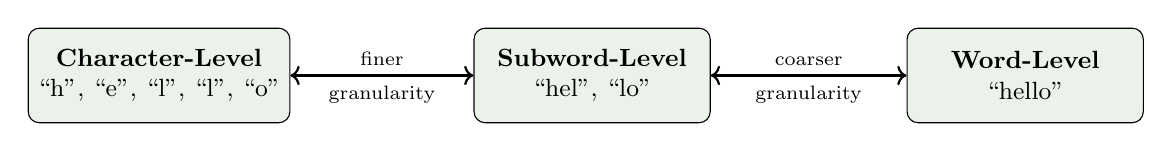
\begin{tikzpicture}[
    box/.style={draw, rounded corners, fill=alfaisalgreen!10, minimum height=1.2cm, minimum width=3cm, font=\small, align=center},
    arr/.style={-{Stealth[length=2.5mm]}, thick}
]
\node[box] (char) at (0,0) {\textbf{Character-Level}\\``h'', ``e'', ``l'', ``l'', ``o''};
\node[box] (sub) at (5.5,0) {\textbf{Subword-Level}\\``hel'', ``lo''};
\node[box] (word) at (11,0) {\textbf{Word-Level}\\``hello''};

\draw[arr, <->] (char) -- node[above, font=\scriptsize] {finer} node[below, font=\scriptsize] {granularity} (sub);
\draw[arr, <->] (sub) -- node[above, font=\scriptsize] {coarser} node[below, font=\scriptsize] {granularity} (word);
\end{tikzpicture}
\end{center}

\begin{itemize}[leftmargin=1.5em]
    \item \textbf{Character-level:} Each character is a token. Tiny vocabulary ($\sim$50--100), but very long sequences.
    \item \textbf{Subword-level:} Words are split into meaningful pieces. Balanced vocabulary ($\sim$30K--100K) and moderate sequence length. \textbf{This is what modern LLMs use.}
    \item \textbf{Word-level:} Each word is a token. Semantically rich, but vocabulary can be huge and OOV is inevitable.
\end{itemize}

\subsection{Why Tokenization Matters for Performance}

The choice of tokenizer directly affects model quality in several ways:

\begin{enumerate}[leftmargin=1.5em]
    \item \textbf{Spelling errors:} Poor tokenizers break misspelled words into meaningless fragments
    \item \textbf{Arithmetic:} How numbers are tokenized affects whether the model can ``see'' individual digits (e.g., ``380'' as one token vs.\ ``3'', ``8'', ``0'')
    \item \textbf{Non-English languages:} Many tokenizers are trained primarily on English; other languages get split into excessively many tokens, reducing quality and increasing cost
    \item \textbf{Inconsistent handling:} The same concept may be tokenized differently depending on context (e.g., leading whitespace, capitalization)
\end{enumerate}

\begin{tcolorbox}[intuitionbox={The Golden Rule}]
\textit{``The better the tokenization, the smarter the model.''} --- A well-designed tokenizer gives the model cleaner, more consistent input, allowing it to focus on learning language patterns rather than fighting tokenization artifacts.
\end{tcolorbox}

% ============================================================
% 5. COMPARING TOKENIZERS: GPT-2 vs GPT-4
% ============================================================
\section{Comparing Tokenizers: GPT-2 vs GPT-4}

OpenAI significantly improved their tokenizer between GPT-2 and GPT-4. Understanding these differences illustrates why tokenizer design matters.

\subsection{Key Differences}

\begin{center}
\renewcommand{\arraystretch}{1.4}
\begin{tabular}{@{}p{4cm}cc@{}}
\toprule
\textbf{Dimension} & \textbf{GPT-2} & \textbf{GPT-4} \\
\midrule
Vocabulary size & $\sim$50,257 & $\sim$100,256 \\
Encoding name & \texttt{r50k\_base} & \texttt{cl100k\_base} \\
Token efficiency & Lower & Higher (fewer tokens for same text) \\
Whitespace handling & Inconsistent & Improved \\
Non-English support & Poor (many tokens per word) & Better (fewer tokens per word) \\
Number handling & Splits inconsistently & More consistent digit handling \\
Special characters & Limited & Better coverage \\
\bottomrule
\end{tabular}
\end{center}

\subsection{Why a Larger Vocabulary Helps}

A larger vocabulary means:
\begin{itemize}[leftmargin=1.5em]
    \item \textbf{Fewer tokens per text} --- common words and phrases become single tokens
    \item \textbf{Shorter sequences} --- reduces computation ($O(n^2)$ attention cost)
    \item \textbf{Better multilingual support} --- room for non-English subwords
    \item \textbf{Lower API cost} --- users pay per token, so efficiency matters
\end{itemize}

\textbf{Trade-off:} A larger vocabulary means a larger embedding matrix, which increases model size and memory usage. The sweet spot for modern LLMs is typically 30K--100K tokens.

\begin{tcolorbox}[questionbox={Self-Check Q2}]
GPT-4's tokenizer uses $\sim$100K tokens while GPT-2 uses $\sim$50K. Why not simply use a vocabulary of 1 million tokens? What would be the disadvantages? \textit{(Solution in Appendix)}
\end{tcolorbox}

% ============================================================
% 6. UNICODE AND WHY IT'S NOT ENOUGH
% ============================================================
\section{Unicode and Why It's Not Enough}

\subsection{What is Unicode?}

Before tokenization, text is represented as a sequence of \textbf{Unicode code points}. Unicode is a universal standard that assigns a unique number to every character in every language:

\begin{center}
\begin{tabular}{@{}lcl@{}}
\toprule
\textbf{Character} & \textbf{Code Point} & \textbf{Description} \\
\midrule
A & U+0041 (65) & Latin capital letter A \\
a & U+0061 (97) & Latin lowercase letter a \\
\textsf{\#} & U+0023 (35) & Number sign \\
{[smiley face]} & U+1F60A (128522) & Smiling face emoji \\
\bottomrule
\end{tabular}
\end{center}

\subsection{Encoding Schemes: UTF-8, UTF-16, UTF-32}

Unicode code points must be encoded as bytes for storage and transmission:

\begin{center}
\renewcommand{\arraystretch}{1.3}
\begin{tabular}{@{}p{2.5cm}p{3cm}p{3cm}p{4cm}@{}}
\toprule
\textbf{Encoding} & \textbf{Bytes/char} & \textbf{Advantage} & \textbf{Disadvantage} \\
\midrule
UTF-8 & 1--4 (variable) & Compact for ASCII/English & Variable-length complicates indexing \\
UTF-16 & 2 or 4 & Good for Asian scripts & Wastes space for ASCII \\
UTF-32 & 4 (fixed) & Simple indexing & Wastes space ($4\times$ ASCII) \\
\bottomrule
\end{tabular}
\end{center}

\subsection{Why Not Use Unicode Code Points as Tokens?}

One might ask: why not simply use each Unicode code point as a token? There are several problems:

\begin{enumerate}[leftmargin=1.5em]
    \item \textbf{Huge vocabulary:} Unicode defines over \textbf{150,000} characters. The embedding matrix would be enormous.
    \item \textbf{Dynamic standard:} New characters (especially emojis) are added regularly. The vocabulary would need constant updating.
    \item \textbf{Long sequences:} Each character becomes a separate token, leading to very long sequences.
    \item \textbf{Quadratic attention cost:} Transformer self-attention is $O(n^2)$ in sequence length---longer sequences are dramatically more expensive.
\end{enumerate}

\subsection{Why Not Use Raw UTF-8 Bytes?}

Another idea: use the 256 possible byte values as the vocabulary. This gives a tiny, fixed vocabulary, but:

\begin{enumerate}[leftmargin=1.5em]
    \item \textbf{Too few tokens:} Only 256 unique tokens---the model has almost no ``vocabulary'' to work with
    \item \textbf{Very long sequences:} A single emoji (e.g., 4 bytes in UTF-8) becomes 4 tokens; words in non-Latin scripts become 2--4 tokens per character
    \item \textbf{No semantic structure:} Individual bytes carry no linguistic meaning
\end{enumerate}

\begin{tcolorbox}[warnbox={The Dilemma}]
Unicode code points: vocabulary too \textbf{large} ($\sim$150K). Raw UTF-8 bytes: vocabulary too \textbf{small} (256). We need something in between---a vocabulary of 30K--100K meaningful \textbf{subword} tokens. This is exactly what BPE and other subword algorithms provide.
\end{tcolorbox}

\begin{tcolorbox}[questionbox={Self-Check Q3}]
If we used raw UTF-8 bytes as our vocabulary (256 tokens), how many tokens would the English word ``hello'' require? How about a Chinese character like ``\,'' (which uses 3 bytes in UTF-8)? What does this tell us about sequence length? \textit{(Solution in Appendix)}
\end{tcolorbox}

% ============================================================
% 7. CHARACTER-LEVEL TOKENIZATION
% ============================================================
\section{Character-Level Tokenization}

\subsection{Definition and Process}

The simplest tokenization strategy: split text into \textbf{individual characters}, including spaces and punctuation. Each unique character becomes a token in the vocabulary.

\subsection{Worked Example: Shakespeare}

Input: \texttt{"To be, or not to be"}

\begin{center}
\texttt{["T", "o", " ", "b", "e", ",", " ", "o", "r", " ", "n", "o", "t", " ", "t", "o", " ", "b", "e"]}
\end{center}

This produces \textbf{19 tokens} from 19 characters (spaces included). In Shakespeare's complete works ($\sim$5 million characters), the vocabulary contains only about \textbf{65 unique characters} (letters, digits, punctuation, whitespace).

\subsection{Advantages}

\begin{itemize}[leftmargin=1.5em]
    \item \textbf{Compact vocabulary:} Only $\sim$50--100 unique tokens (for English). The embedding matrix is tiny.
    \item \textbf{Language-independent:} Works for any language without language-specific preprocessing.
    \item \textbf{No OOV problem:} Any text can be represented---there are no unknown characters.
    \item \textbf{Captures subword patterns:} The model can learn morphological patterns (e.g., ``-ing'', ``-ed'', ``un-'') from raw characters.
\end{itemize}

\subsection{Disadvantages}

\begin{itemize}[leftmargin=1.5em]
    \item \textbf{Very long sequences:} A 500-word paragraph might produce 3,000+ character tokens.
    \item \textbf{Quadratic attention cost:} Self-attention is $O(n^2)$. Doubling sequence length quadruples the cost.
    \item \textbf{No semantic structure:} Individual characters carry no meaning. The model must learn that ``c'', ``a'', ``t'' together mean a feline---a much harder learning task.
    \item \textbf{Slower training:} More tokens per example means more computation per training step.
\end{itemize}

\begin{tcolorbox}[intuitionbox={When to Use Character-Level Tokenization}]
Character-level models are best for tasks where \textbf{character patterns matter}: spelling correction, handwriting recognition, transliteration, or processing languages with very large character sets (e.g., Chinese). They are generally \textbf{not used} for large-scale language models due to sequence length constraints.
\end{tcolorbox}

% ============================================================
% 8. WORD-LEVEL TOKENIZATION
% ============================================================
\section{Word-Level Tokenization}

\subsection{Definition and Process}

Split text on whitespace and punctuation boundaries. Each unique word becomes a token in the vocabulary.

\subsection{Worked Example: Shakespeare}

Input: \texttt{"To be, or not to be"}

\begin{center}
\texttt{["To", "be", ",", "or", "not", "to", "be"]}
\end{center}

This produces \textbf{7 tokens}---much fewer than the 19 character tokens. However, Shakespeare's complete works contain approximately \textbf{30,000 unique words}---a much larger vocabulary.

\subsection{Advantages}

\begin{itemize}[leftmargin=1.5em]
    \item \textbf{Captures word semantics:} Each token is a meaningful linguistic unit. The model can directly learn word meanings.
    \item \textbf{Shorter sequences:} Far fewer tokens per text, enabling longer context windows.
    \item \textbf{Intuitive:} Aligns with how humans think about language.
\end{itemize}

\subsection{Disadvantages}

\begin{itemize}[leftmargin=1.5em]
    \item \textbf{Large vocabulary:} English alone has 170,000+ words; technical domains add more. The embedding matrix becomes enormous.
    \item \textbf{OOV problem:} New words, misspellings, and rare terms cannot be represented.
    \item \textbf{Morphological blindness:} The model treats ``run'', ``running'', ``runner'', and ``runs'' as \emph{completely unrelated} tokens, wasting capacity learning the same root meaning four times.
    \item \textbf{Language-dependent:} Whitespace-based splitting does not work for Chinese, Japanese, Thai, and other languages without word boundaries.
\end{itemize}

\begin{tcolorbox}[warnbox={The Core Trade-off}]
Character-level tokenization: small vocabulary, long sequences, no semantics.\\
Word-level tokenization: large vocabulary, short sequences, rich semantics but OOV issues.\\[4pt]
\textbf{Can we get the best of both worlds?} Yes---with \textbf{subword tokenization}.
\end{tcolorbox}

\begin{tcolorbox}[questionbox={Self-Check Q4}]
Consider the words ``run'', ``running'', ``runner'', and ``runs''. Explain why word-level tokenization wastes model capacity for these words, and how subword tokenization would handle them more efficiently. \textit{(Solution in Appendix)}
\end{tcolorbox}

% ============================================================
% 9. SUBWORD TOKENIZATION
% ============================================================
\section{Subword Tokenization: The Best of Both Worlds}

\subsection{Why Subword Tokenization?}

We have seen two extremes:
\begin{itemize}[leftmargin=1.5em]
    \item \textbf{Characters:} Too fine-grained---sequences too long, no semantics.
    \item \textbf{Words:} Too coarse---vocabulary too large, OOV problem.
\end{itemize}

Subword tokenization \textbf{bridges the gap}. The goals are:

\begin{enumerate}[leftmargin=1.5em]
    \item \textbf{Optimize vocabulary size:} Keep it manageable (30K--100K tokens)
    \item \textbf{Eliminate OOV:} Any word can be decomposed into known subwords
    \item \textbf{Represent morphemes:} Capture meaningful sub-units like prefixes, suffixes, and roots
\end{enumerate}

\subsection{How It Works (Intuition)}

Common words (``the'', ``is'', ``and'') are kept as single tokens. Rare or complex words are split into smaller pieces:

\begin{center}
\renewcommand{\arraystretch}{1.3}
\begin{tabular}{@{}ll@{}}
\toprule
\textbf{Word} & \textbf{Subword Tokens} \\
\midrule
\texttt{unhappiness} & \texttt{["un", "happiness"]} or \texttt{["un", "happ", "iness"]} \\
\texttt{tokenization} & \texttt{["token", "ization"]} \\
\texttt{transformer} & \texttt{["transform", "er"]} \\
\texttt{xylophone} & \texttt{["x", "yl", "ophone"]} \\
\bottomrule
\end{tabular}
\end{center}

\subsection{Arabic: A Case for Morphological Awareness}

Arabic is a \textbf{morphologically rich} language built on a root-and-pattern system. The triliteral root \textbf{k-t-b} (related to writing) generates many words:

\begin{center}
\renewcommand{\arraystretch}{1.3}
\begin{tabular}{@{}lll@{}}
\toprule
\textbf{Arabic Word} & \textbf{Transliteration} & \textbf{Meaning} \\
\midrule
kataba & kataba & he wrote \\
kaatib & kaatib & writer \\
kitaab & kitaab & book \\
kutub & kutub & books \\
katabtu & katabtu & I wrote \\
maktaba & maktaba & library \\
\bottomrule
\end{tabular}
\end{center}

A good subword tokenizer can learn to recognize the shared root \texttt{ktb} across all these forms, enabling the model to transfer knowledge between related words. Word-level tokenization would treat each form as an independent, unrelated token.

\begin{tcolorbox}[intuitionbox={Key Insight}]
Subword tokenization is not just an engineering trick---it captures \textbf{linguistic structure}. Morphemes (the smallest meaningful units) are naturally discovered by the algorithm, enabling the model to generalize across word forms.
\end{tcolorbox}

% ============================================================
% 10. BYTE PAIR ENCODING (BPE)
% ============================================================
\section{Byte Pair Encoding (BPE)}

\subsection{The Algorithm}

BPE is the most widely used subword tokenization algorithm. It was originally a data compression technique (Gage, 1994) and was adapted for NLP by Sennrich et al.\ (2016). The algorithm is elegant in its simplicity:

\begin{tcolorbox}[colback=white, colframe=alfaisalgreen, boxrule=0.5pt, title={\textbf{BPE Algorithm}}]
\begin{enumerate}[leftmargin=1.5em]
    \item Start with a vocabulary of all individual characters (or bytes)
    \item Count all consecutive pairs of tokens in the training corpus
    \item Find the most frequent pair
    \item Merge that pair into a new single token; add it to the vocabulary
    \item Repeat steps 2--4 until the desired vocabulary size is reached
\end{enumerate}
\end{tcolorbox}

\subsection{Worked Example: ``low lower lowest''}

Let us trace through BPE step by step.

\medskip\noindent\textbf{Initial state:} Represent each word as a sequence of characters (using byte values for clarity):

\begin{lstlisting}
"low"    -> [108, 111, 119]           # l, o, w
"lower"  -> [108, 111, 119, 101, 114] # l, o, w, e, r
"lowest" -> [108, 111, 119, 101, 115, 116] # l, o, w, e, s, t
\end{lstlisting}

Initial vocabulary: all unique bytes appearing in the corpus.

\begin{tcolorbox}[colback=white, colframe=alfaisalgreen, boxrule=0.5pt, title={\textbf{Merge 1 --- Most frequent pair: (108, 111) = ``lo''}}]
The pair \texttt{(108, 111)} (i.e., ``l'' followed by ``o'') appears 3 times (once in each word). This is the most frequent pair.

\textbf{Action:} Create a new token 256 = ``lo''. Replace all occurrences:
\begin{lstlisting}
"low"    -> [256, 119]           # lo, w
"lower"  -> [256, 119, 101, 114] # lo, w, e, r
"lowest" -> [256, 119, 101, 115, 116] # lo, w, e, s, t
\end{lstlisting}
Vocabulary size: original bytes + 1 new token.
\end{tcolorbox}

\begin{tcolorbox}[colback=white, colframe=alfaisalgreen, boxrule=0.5pt, title={\textbf{Merge 2 --- Most frequent pair: (256, 119) = ``low''}}]
The pair \texttt{(256, 119)} (i.e., ``lo'' followed by ``w'') appears 3 times.

\textbf{Action:} Create a new token 257 = ``low''. Replace all occurrences:
\begin{lstlisting}
"low"    -> [257]                # low
"lower"  -> [257, 101, 114]     # low, e, r
"lowest" -> [257, 101, 115, 116] # low, e, s, t
\end{lstlisting}
\end{tcolorbox}

\begin{tcolorbox}[colback=white, colframe=alfaisalgreen, boxrule=0.5pt, title={\textbf{Merge 3 --- Most frequent pair: (257, 101) = ``lowe''}}]
The pair \texttt{(257, 101)} (i.e., ``low'' followed by ``e'') appears 2 times (in ``lower'' and ``lowest'').

\textbf{Action:} Create a new token 258 = ``lowe''. Replace all occurrences:
\begin{lstlisting}
"low"    -> [257]             # low
"lower"  -> [258, 114]       # lowe, r
"lowest" -> [258, 115, 116]  # lowe, s, t
\end{lstlisting}
\end{tcolorbox}

The process continues until the target vocabulary size is reached. Notice how BPE naturally discovers meaningful subword units: ``low'' becomes a single token, and ``lower'' and ``lowest'' share the common prefix ``lowe''.

\subsection{BPE in GPT-2: Byte-Level BPE}

GPT-2 uses a variant called \textbf{byte-level BPE}:

\begin{enumerate}[leftmargin=1.5em]
    \item \textbf{Base vocabulary:} 256 raw UTF-8 byte values (not Unicode characters). This ensures \emph{any} text can be tokenized---no \texttt{<UNK>} tokens needed.
    \item \textbf{Regex pre-splitting:} Before applying BPE merges, the text is split using a regex pattern that separates:
    \begin{itemize}[leftmargin=1em]
        \item Words (with optional leading space)
        \item Numbers
        \item Punctuation
        \item Whitespace sequences
    \end{itemize}
    \item \textbf{No cross-category merges:} BPE merges are only applied \emph{within} each regex-matched chunk. This prevents nonsensical merges like merging a letter with a digit or merging across word boundaries.
\end{enumerate}

\begin{lstlisting}[language=Python]
# GPT-2 regex pattern (simplified)
import regex
pattern = r"""'s|'t|'re|'ve|'m|'ll|'d
| ?\p{L}+
| ?\p{N}+
| ?[^\s\p{L}\p{N}]+
| \s+"""
\end{lstlisting}

\begin{tcolorbox}[intuitionbox={Why Byte-Level?}]
By starting from bytes instead of Unicode characters, GPT-2 can tokenize \textbf{any text in any language or encoding} without ever producing an unknown token. The 256-byte base vocabulary is universal, compact, and fixed. BPE merges then build up from bytes to meaningful subword units.
\end{tcolorbox}

\begin{tcolorbox}[questionbox={Self-Check Q5}]
In BPE, why do we merge the most \emph{frequent} pair at each step? What would happen if we instead merged the \emph{least} frequent pair? \textit{(Solution in Appendix)}
\end{tcolorbox}

% ============================================================
% 11. TIKTOKEN LIBRARY
% ============================================================
\section{TikToken: OpenAI's Tokenization Library}

\textbf{TikToken} is OpenAI's official, open-source tokenization library used in GPT-2, GPT-3, GPT-3.5, and GPT-4. It provides fast, production-grade BPE tokenization.

\subsection{Basic Usage}

\begin{lstlisting}[language=Python]
import tiktoken

# Load GPT-4's tokenizer
enc = tiktoken.encoding_for_model("gpt-4")

# Encode text to token IDs
tokens = enc.encode("Hello, world!")
print(tokens)   # e.g., [9906, 11, 1917, 0]

# Decode token IDs back to text
text = enc.decode(tokens)
print(text)     # "Hello, world!"

# Count tokens (useful for API cost estimation)
num_tokens = len(enc.encode("Your text here"))
\end{lstlisting}

\subsection{Comparing Encodings}

\begin{center}
\renewcommand{\arraystretch}{1.3}
\begin{tabular}{@{}llc@{}}
\toprule
\textbf{Encoding} & \textbf{Used by} & \textbf{Vocab Size} \\
\midrule
\texttt{r50k\_base} & GPT-2 & 50,257 \\
\texttt{p50k\_base} & GPT-3 (Codex) & 50,281 \\
\texttt{cl100k\_base} & GPT-3.5, GPT-4 & 100,256 \\
\bottomrule
\end{tabular}
\end{center}

\begin{tcolorbox}[warnbox={Practical Tip}]
When using OpenAI's API, you \textbf{pay per token}. Use TikToken locally to estimate costs \emph{before} making API calls. Different models use different tokenizers, so always match the encoding to the model you plan to use.
\end{tcolorbox}

\begin{tcolorbox}[questionbox={Self-Check Q6}]
Using TikToken, the sentence ``I love deep learning'' is encoded as 4 tokens by GPT-4's tokenizer. If the same sentence is encoded by GPT-2's tokenizer, would you expect more tokens, fewer tokens, or the same number? Explain your reasoning. \textit{(Solution in Appendix)}
\end{tcolorbox}

% ============================================================
% 12. SUMMARY: CHOOSING THE RIGHT TOKENIZATION
% ============================================================
\section{Summary: Choosing the Right Tokenization}

\subsection{Comparison Table}

\begin{center}
\renewcommand{\arraystretch}{1.4}
\begin{tabular}{@{}p{3.2cm}p{3.5cm}p{3.5cm}p{3.5cm}@{}}
\toprule
\textbf{Dimension} & \textbf{Character-Level} & \textbf{Word-Level} & \textbf{Subword (BPE)} \\
\midrule
Vocabulary size & Very small ($\sim$50--100) & Very large ($\sim$100K+) & Moderate ($\sim$30K--100K) \\
Sequence length & Very long & Short & Moderate \\
OOV handling & No OOV & Frequent OOV & No OOV \\
Semantic content & None per token & Rich per token & Moderate per token \\
Morphology & Must learn from scratch & Ignores it & Captures naturally \\
Computation cost & High ($O(n^2)$ with long $n$) & Low & Moderate \\
Used in practice & Specialized tasks & Legacy systems & \textbf{All modern LLMs} \\
\bottomrule
\end{tabular}
\end{center}

\subsection{The Evolution}

\begin{center}
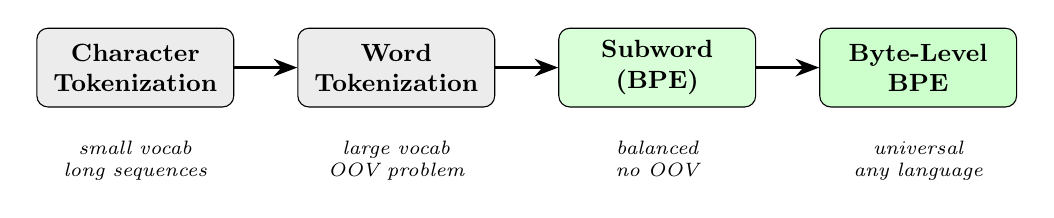
\begin{tikzpicture}[
    node distance=0.8cm,
    box/.style={draw, rounded corners, minimum height=1cm, minimum width=2.5cm, font=\small\bfseries, align=center},
    arr/.style={-{Stealth[length=3mm]}, thick}
]
\node[box, fill=gray!15] (char) {Character\\Tokenization};
\node[box, fill=gray!15, right=of char] (word) {Word\\Tokenization};
\node[box, fill=green!15, right=of word] (sub) {Subword\\(BPE)};
\node[box, fill=green!20, right=of sub] (byte) {Byte-Level\\BPE};

\draw[arr] (char) -- (word);
\draw[arr] (word) -- (sub);
\draw[arr] (sub) -- (byte);

\node[below=0.3cm, font=\scriptsize\itshape, text width=2.5cm, align=center] at (char.south) {small vocab\\long sequences};
\node[below=0.3cm, font=\scriptsize\itshape, text width=2.5cm, align=center] at (word.south) {large vocab\\OOV problem};
\node[below=0.3cm, font=\scriptsize\itshape, text width=2.5cm, align=center] at (sub.south) {balanced\\no OOV};
\node[below=0.3cm, font=\scriptsize\itshape, text width=2.5cm, align=center] at (byte.south) {universal\\any language};
\end{tikzpicture}
\end{center}

\begin{tcolorbox}[intuitionbox={Bottom Line}]
Modern language models universally use \textbf{subword tokenization} (specifically byte-level BPE or similar algorithms like SentencePiece). This gives the optimal trade-off between vocabulary size, sequence length, and linguistic coverage. If you are building or fine-tuning an LLM, the tokenizer is not an afterthought---it is a \textbf{design decision} that directly impacts model quality.
\end{tcolorbox}

\begin{tcolorbox}[questionbox={Self-Check Q7}]
You are designing a tokenizer for a multilingual model that must support English, Arabic, Chinese, and code. Would you choose character-level, word-level, or subword tokenization? Justify your choice by addressing each language's specific challenges. \textit{(Solution in Appendix)}
\end{tcolorbox}

% ============================================================
% APPENDIX
% ============================================================
\newpage
\section*{Appendix: Solutions to Self-Check Questions}
\addcontentsline{toc}{section}{Appendix: Solutions to Self-Check Questions}

\subsection*{Q1: Why is mapping all unknown words to \texttt{<UNK>} problematic?}

When all unknown words map to the same \texttt{<UNK>} token, the model \textbf{loses all ability to distinguish} between them. For example, consider a medical NLP system with a limited vocabulary:

\begin{itemize}[leftmargin=1.5em]
    \item \texttt{"The patient has \textbf{pneumonia}"} $\to$ \texttt{["The", "patient", "has", "<UNK>"]}
    \item \texttt{"The patient has \textbf{diabetes}"} $\to$ \texttt{["The", "patient", "has", "<UNK>"]}
\end{itemize}

Both sentences produce \emph{identical} token sequences. The model cannot distinguish between pneumonia and diabetes---a potentially dangerous failure. Subword tokenization would split these into recognizable pieces (\texttt{"pneum", "onia"} and \texttt{"diab", "etes"}), preserving distinguishing information.

\subsection*{Q2: Why not use a vocabulary of 1 million tokens?}

A vocabulary of 1 million tokens would cause several problems:

\begin{enumerate}[leftmargin=1.5em]
    \item \textbf{Enormous embedding matrix:} With embedding dimension 768 (like GPT-2), the embedding layer alone would have $1{,}000{,}000 \times 768 \approx 768$ million parameters---nearly as many as the entire GPT-2 model.
    \item \textbf{Data sparsity:} Most tokens would appear very rarely in training data, leading to poorly trained embeddings for rare tokens.
    \item \textbf{Overfitting:} The model memorizes rare token patterns instead of learning generalizable subword structure.
    \item \textbf{Diminishing returns:} Beyond $\sim$100K tokens, additional vocabulary entries provide minimal compression benefit while significantly increasing model size.
\end{enumerate}

The sweet spot ($\sim$30K--100K) balances compression efficiency against embedding quality and model size.

\subsection*{Q3: UTF-8 byte tokenization of ``hello'' and a Chinese character}

\textbf{``hello'':} Each ASCII character is 1 byte in UTF-8, so ``hello'' = 5 bytes = \textbf{5 tokens}. This is identical to character-level tokenization for English.

\textbf{A Chinese character:} Most Chinese characters use \textbf{3 bytes} in UTF-8. So a single meaningful character becomes \textbf{3 tokens}. A 10-character Chinese sentence would become 30 tokens.

\textbf{Implication:} Raw UTF-8 byte tokenization creates \textbf{extremely long sequences} for non-English text, making it impractical. A 500-character Chinese text would become 1,500 byte tokens, dramatically increasing attention computation ($O(n^2)$). This is why we need BPE to merge frequent byte sequences into meaningful subword tokens.

\subsection*{Q4: Word-level tokenization and morphological waste}

With word-level tokenization, ``run'', ``running'', ``runner'', and ``runs'' are four \textbf{completely independent} tokens with four separate embedding vectors. The model must learn from scratch that these words share the concept of ``run''---it gets no help from the tokenizer.

With subword tokenization (BPE), these would be tokenized as:
\begin{itemize}[leftmargin=1.5em]
    \item \texttt{"run"} $\to$ \texttt{["run"]}
    \item \texttt{"running"} $\to$ \texttt{["run", "ning"]}
    \item \texttt{"runner"} $\to$ \texttt{["run", "ner"]}
    \item \texttt{"runs"} $\to$ \texttt{["run", "s"]}
\end{itemize}

All four words share the token \texttt{"run"}, so the model \textbf{automatically} transfers knowledge between them. The suffixes \texttt{"ning"}, \texttt{"ner"}, and \texttt{"s"} are also shared across many other words (e.g., ``planning'', ``trainer'', ``cats''), further improving generalization.

\subsection*{Q5: Why merge the most frequent pair in BPE?}

Merging the most frequent pair is a \textbf{greedy compression strategy}: at each step, we create the token that \textbf{reduces the total sequence length the most}. Frequent pairs appear many times, so merging them eliminates the most tokens from the corpus.

If we merged the \textbf{least} frequent pair instead:
\begin{itemize}[leftmargin=1.5em]
    \item We would create tokens that appear only once or twice in the corpus
    \item The vocabulary would fill up with \textbf{rare, overly specific} tokens (e.g., merging ``x'' and ``q'' because they co-occur once)
    \item Common patterns (like ``th'', ``in'', ``er'') would never get merged because they would always be outranked by some rare pair
    \item The resulting tokenization would be \textbf{inefficient}: common words would still be split into many characters, while rare words get special tokens they do not deserve
\end{itemize}

The frequency-based approach ensures the vocabulary captures the most \textbf{useful} patterns first.

\subsection*{Q6: Token count comparison between GPT-2 and GPT-4 tokenizers}

You would generally expect GPT-2's tokenizer to produce the \textbf{same number or more tokens} for ``I love deep learning'':

\begin{itemize}[leftmargin=1.5em]
    \item GPT-4's tokenizer (\texttt{cl100k\_base}) has \textbf{twice the vocabulary} of GPT-2's (\texttt{r50k\_base})
    \item A larger vocabulary means more common words and phrases are stored as single tokens
    \item Common English phrases like ``deep learning'' might be a single token in GPT-4 but two tokens in GPT-2
\end{itemize}

In this specific case, ``I love deep learning'' contains common English words, so both tokenizers may produce a similar count. But for longer or more varied text, GPT-4 consistently produces \textbf{fewer tokens}, which is one reason it is more cost-efficient.

\subsection*{Q7: Choosing a tokenizer for a multilingual + code model}

\textbf{Subword tokenization (byte-level BPE)} is the clear choice. Here is why, language by language:

\begin{itemize}[leftmargin=1.5em]
    \item \textbf{English:} Subword handles morphology naturally (``un'' + ``happy'' + ``ness''). Word-level would create OOV for rare terms; character-level would create unnecessarily long sequences.

    \item \textbf{Arabic:} The root-and-pattern morphology (e.g., k-t-b family) is naturally captured by subword units. Word-level would treat each inflected form as independent, missing the shared root structure. Character-level would work but create very long sequences.

    \item \textbf{Chinese:} Has no whitespace between words, so word-level tokenization requires a separate word segmentation step. Byte-level BPE handles this naturally---common characters and character combinations become single tokens through merges.

    \item \textbf{Code:} Programming languages have consistent syntactic patterns (keywords, operators, indentation). BPE learns these patterns and creates tokens for common constructs (\texttt{def}, \texttt{return}, \texttt{==}). Character-level would make code sequences extremely long; word-level would fail on variable names and nested syntax.
\end{itemize}

The byte-level variant is essential: it starts from 256 bytes, so it can handle \textbf{any encoding} without unknown tokens. This is exactly why GPT-4 uses byte-level BPE with a 100K vocabulary.

\end{document}
